\documentclass[11pt,reqno]{amsart}

\usepackage[T1]{fontenc}
\usepackage{lmodern}
\usepackage[utf8]{inputenc}
\usepackage{amsmath,amssymb,amsthm,mathrsfs}
\usepackage{enumitem}
\usepackage{microtype}
\usepackage{tikz}
\usetikzlibrary{calc,decorations.pathmorphing,patterns}
\usepackage[colorlinks=true,linkcolor=blue!50!black,citecolor=blue!50!black,urlcolor=blue!50!black]{hyperref}

\setlength{\textwidth}{6.3in}
\setlength{\oddsidemargin}{0.1in}
\setlength{\evensidemargin}{0.1in}
\setlength{\textheight}{8.7in}
\setlength{\topmargin}{-0.1in}

\theoremstyle{plain}
\newtheorem{theorem}{Theorem}[section]
\newtheorem{lemma}[theorem]{Lemma}
\newtheorem{proposition}[theorem]{Proposition}
\newtheorem{corollary}[theorem]{Corollary}
\theoremstyle{definition}
\newtheorem{definition}[theorem]{Definition}
\newtheorem{example}[theorem]{Example}
\newtheorem{question}[theorem]{Question}
\theoremstyle{remark}
\newtheorem{remark}[theorem]{Remark}

\newcommand{\D}{\mathcal{D}}
\newcommand{\F}{\mathscr{F}}
\newcommand{\M}{\mathcal{M}}
\newcommand{\PP}{\mathcal{P}}
\newcommand{\cl}{\operatorname{cl}}
\newcommand{\intr}{\operatorname{int}}
\newcommand{\bd}{\operatorname{bd}}
\newcommand{\diam}{\operatorname{diam}}
\newcommand{\Ls}{\operatorname{Ls}}
\newcommand{\N}{\mathbb{N}}
\newcommand{\Q}{\mathbb{Q}}
\newcommand{\R}{\mathbb{R}}
\newcommand{\cc}{\mathfrak{c}}
\newcommand{\rd}{\ominus}

\begin{document}

\title[Countable hyperspaces of regular subcontinua]{On the structure of countable hyperspaces of regular subcontinua}

\author{Lucas Alves de Almeida}
\address{Independent Researcher}
\email{lucasderiva2x@gmail.com}

\date{November 11, 2026}

\subjclass[2020]{Primary 54F16; Secondary 54B20, 54F15, 54H05}
\keywords{Continuum, hyperspace, regular subcontinuum, regular closed set, rational numbers, scattered space, Baire category, formalization, Lean}

\begin{abstract}
Let $X$ be a metric continuum and let $\D(X)$ be its hyperspace of regular subcontinua, that is, of the subcontinua of $X$ which are the closure of their interior. We prove that if $\D(X)$ is countable, then the interiors of its minimal elements are dense in $X$, and every regular subcontinuum is determined by the minimal elements it contains. We further establish that $\D(X)$ is a $G_\delta$ subset of the hyperspace $C(X)$ of subcontinua whenever $X$ admits a family of regular subcontinua whose interiors have dense union and which satisfies an absorption property. Consequently, every countable $\D(X)$ is completely metrizable and scattered. In particular, $\D(X)$ is never homeomorphic to the rational numbers, which answers a question of Ram\'irez Angarita and of Camargo, Ordo\~nez and Ram\'irez. The theorems of the paper are formalized in Lean~4.
\end{abstract}

\maketitle

\section{Introduction}

\subsection{The problem}
A \emph{continuum} is a nonempty compact connected metric space. For a continuum $X$, the hyperspace $C(X)$ of all subcontinua of $X$, with the Hausdorff metric, is a classical object~\cite{IN}. In 2018 Ordo\~nez~\cite{Ord18} introduced a subspace of $C(X)$ which records the subcontinua that are ``thick everywhere'': a subcontinuum $A$ of $X$ is \emph{regular} if $A=\cl\intr A$, and
\[
\D(X)=\{A\in C(X): A=\cl\intr A\}
\]
is the \emph{hyperspace of regular subcontinua} of $X$. Always $X\in\D(X)$.

The space $\D(X)$ behaves very differently from $C(X)$. It need not be compact or connected, and its size is sensitive to the fine structure of $X$. If $X$ is locally connected, $\D(X)$ is dense in $C(X)$, arcwise connected and contractible \cite[Theorem~3.6]{Ord18}. A continuum is \emph{indecomposable} if it is not the union of two proper subcontinua; equivalently, every proper subcontinuum has empty interior. If $X$ is indecomposable, then $\D(X)=\{X\}$. Between these extremes, $\D(X)$ is compact if and only if it is finite \cite[Corollary~4.13]{Ord18}. This led to the problem of deciding which spaces arise as $\D(X)$ \cite[Problem~3.22]{CORa}. Further properties of $\D(X)$, and its interplay with the hyperspace of subcontinua with empty interior, are studied in~\cite{Ord21,CORa}.

Several cases are known. Camargo, Ordo\~nez and Ram\'irez showed that $|\D(X)|\notin\{2,4,5,8,9\}$ \cite[Proposition~3.18]{CORa} and that $\D(X)$ is never homeomorphic to the discrete space $\N$ \cite[Theorem~3.25]{CORa}; the finite cardinalities that do occur are determined in~\cite{AdAfin}. Ram\'irez Angarita gave a continuum with $\D(X)$ homeomorphic to the ordinal space $\omega^2$ \cite[Ejemplo~3.2.1]{Ram23}, and showed that $\D(X)$ is always a $\boldsymbol{\Pi}^0_3$ subset of $C(X)$ \cite[Teorema~2.0.2]{Ram23}. The following question appears in \cite[Pregunta~3.2.14]{Ram23} and in \cite[Question~3.26]{CORa}.

\begin{question}[Ram\'irez Angarita; Camargo, Ordo\~nez and Ram\'irez]\label{Q:main}
Does there exist a continuum $X$ such that $\D(X)$ is homeomorphic to either the rationals $\Q$ or the irrationals?
\end{question}

The irrational half was answered positively in~\cite{AdAirr}, where a continuum $X\subseteq\ell^2$ with $\D(X)$ homeomorphic to the Baire space $\N^{\N}$ is constructed; that paper leaves the rational half open. By Sierpi\'nski's theorem \cite[Exercise~7.12]{Kechris}, a space is homeomorphic to $\Q$ exactly when it is nonempty, countable, metrizable and has no isolated points. So the rational half asks for a continuum whose family of regular subcontinua is countably infinite and has no isolated point in the Hausdorff metric.

\subsection{Why the rational case is different}
The examples above are built from indecomposable continua glued along small sets. In such a continuum each indecomposable piece acts as an indivisible unit, and a regular subcontinuum is determined by the pieces it contains. Two mechanisms are then available, and each fails for $\Q$ in a different way. If small pieces are attached \emph{independently} to a fixed regular subcontinuum, every subfamily of them can be added, so there are continuum many regular subcontinua. If they are attached in a \emph{nested} way, as in the example with $\D(X)\cong\omega^2$, the hyperspace stays countable but finite configurations are isolated points. There is also a descriptive obstruction: a space homeomorphic to $\Q$ is not completely metrizable, so $\D(X)$ would have to fail to be a $G_\delta$ subset of the compact space $C(X)$, whereas the coding used in~\cite{AdAirr} always produces a $G_\delta$ set.

These observations do not exclude a continuum of a completely different nature, in which regular subcontinua are not assembled from indivisible pieces at all. The difficulty of the rational case is to control \emph{every} metric continuum with a countable hyperspace of regular subcontinua. The content of this paper is that countability alone forces the piecewise structure.

\subsection{Results}
The first result is the answer to the rational half of Question~\ref{Q:main}. Recall that a space is \emph{scattered} if each of its nonempty subspaces has an isolated point.

\begin{theorem}[Main Theorem]\label{T:main}
Let $X$ be a metric continuum such that $\D(X)$ is countable. Then $\D(X)$ is a $G_\delta$ subset of $C(X)$. Consequently $\D(X)$ is completely metrizable and scattered, and its isolated points form a dense subset. In particular there is no metric continuum $X$ such that $\D(X)$ is homeomorphic to $\Q$.
\end{theorem}

Since $\D(X)$ is a Borel subset of $C(X)$ \cite[Teorema~2.0.2]{Ram23}, it is either countable or of cardinality $\cc$ \cite[Theorem~13.6]{Kechris}. Theorem~\ref{T:main} therefore says that $\D(X)$ is either of cardinality $\cc$ or a scattered, completely metrizable countable space.

\begin{remark}\label{R:complete}
``Completely metrizable'' means that \emph{some} complete metric induces the topology of $\D(X)$. It does not mean that the Hausdorff metric is complete on $\D(X)$, and in the infinite case it never is: a subspace on which the Hausdorff metric is complete is closed in the compact space $C(X)$, hence compact, whereas $\D(X)$ is compact only if it is finite \cite[Corollary~4.13]{Ord18}. So there is no conflict between Theorem~\ref{T:main} and that result. In Example~\ref{E:chain} the regular subcontinua $K_n$ converge in $C(X)$ to the singleton $\{p\}$, which is not in $\D(X)$.
\end{remark}

The Main Theorem is a consequence of two results of independent interest. An element $N$ of $\D(X)$ is \emph{minimal} if no element of $\D(X)$ is properly contained in $N$.

\begin{theorem}[Structure Theorem]\label{T:structure}
Let $X$ be a metric continuum such that $\D(X)$ is countable, and let $\M$ be the set of minimal elements of $\D(X)$.
\begin{enumerate}[label=\textup{(\arabic*)}]
\item\label{S1} \textup{(Absorption)} If $A\in\D(X)$ and $N\in\M$, then either $N\subseteq A$ or $N\cap\intr A=\emptyset$.
\item\label{S2} Distinct elements of $\M$ have disjoint interiors.
\item\label{S3} \textup{(Density)} The union of the interiors of the elements of $\M$ is dense in $X$.
\item\label{S4} Every $A\in\D(X)$ is the closure of the union of the elements of $\M$ contained in $A$; in particular $A$ contains a minimal element.
\end{enumerate}
\end{theorem}

Part~\ref{S1} extends \cite[Proposition~3.15]{CORa}, which is the same statement under the stronger hypothesis that $\D(X)$ is discrete (a discrete subspace of the separable metric space $C(X)$ is countable). Parts~\ref{S2}--\ref{S4} extend to countable $\D(X)$ the description of finite $\D(X)$ in \cite[Theorem~3.16]{CORa}, where $X$ is a finite union of minimal elements with pairwise disjoint interiors. Countability cannot be dropped: the arc has no minimal regular subcontinuum, and Example~\ref{E:cone} gives a continuum with a minimal regular subcontinuum for which absorption fails.

We call a continuum \emph{$\D$-atomic} if it has a family of regular subcontinua with the absorption property whose interiors have dense union (Definition~\ref{D:atomic}). Theorem~\ref{T:structure} says that a continuum with countable $\D(X)$ is $\D$-atomic. The second ingredient needs no cardinality assumption.

\begin{theorem}\label{T:Gdelta}
If $X$ is a $\D$-atomic continuum, then $\D(X)$ is a $G_\delta$ subset of $C(X)$.
\end{theorem}

\subsection{The proof strategy}
Countability of $\D(X)$ is used through three different mechanisms, and it is worth separating them.

The first concerns \emph{additions} (Lemma~\ref{L:independent}): if infinitely many regular subcontinua $C_n$ meet a fixed regular subcontinuum $A$, and each $C_n$ has a point which is not approximated by $A$ and the other $C_m$, then $\Theta\mapsto\cl(A\cup\bigcup_{n\in\Theta}C_n)$ is an injection of the power set of $\N$ into $\D(X)$. A countable $\D(X)$ admits no such \emph{independent family}. The second concerns \emph{deletions} (Theorem~\ref{T:blister}): if infinitely many pairwise disjoint open sets can be removed from a regular subcontinuum in every finite combination, leaving a regular subcontinuum each time, then suitable infinite combinations can be removed as well, and again $|\D(X)|=\cc$. The third is a direct use of an enumeration of $\D(X)$: it produces a tree of finite covers of $X$, countability bounds the number of branches of this tree, and the Baire category theorem then applies to the resulting countable closed cover.

No one of these mechanisms does the work of the others. The arc has no independent family and no infinite family of removable open sets, and yet it has continuum many regular subcontinua and no minimal one (Remark~\ref{R:arc}). The proof proceeds in five steps.

\begin{enumerate}[label=\textup{(\roman*)}]
\item \emph{Complements.} For $A,B\in\D(X)$ the \emph{regularised difference} $B\rd A=\cl(\intr B\setminus A)$ has finitely many components, each a regular subcontinuum (Lemma~\ref{L:complement}). Infinitely many components would give an independent family over $A$; this is the only step that uses the first mechanism. It yields absorption at once: if $N$ is minimal and $N\not\subseteq A$, a component of $N\rd A$ is a regular subcontinuum inside $N$, hence equals $N$, and $N\rd A$ misses $\intr A$.
\item \emph{An algebra.} It follows that the finite unions of regular subcontinua are closed under the Boolean operations of the algebra of regular closed sets (Proposition~\ref{P:algebra}). Any regular subcontinuum can then be cut along any other into finitely many regular subcontinua.
\item \emph{Decreasing intersections.} The intersection of a decreasing sequence of regular subcontinua need not be regular. We show that, when $\D(X)$ is countable, it is regular wherever it has interior: the closure of the interior of the intersection is a finite union of regular subcontinua (Lemma~\ref{L:decreasing}). Here the counting is done by the second mechanism: if the complement of the intersection had infinitely many components, one could construct infinitely many removable open sets (``blisters'').
\item \emph{Density.} This is the third mechanism. Enumerate $\D(X)=\{D_1,D_2,\dots\}$ and cut $X$ successively along $D_1,D_2,\dots$. This gives a tree of finite covers by regular subcontinua. Ordering each cover so that its initial unions are connected shows that the tree has only countably many branches. The intersections along the branches form a countable closed cover of $X$, and a branch intersection with nonempty interior is a minimal element of $\D(X)$. The Baire category theorem gives density (Theorem~\ref{T:density}).
\item \emph{Complexity.} For a $\D$-atomic continuum, membership of a subcontinuum in $\D(X)$ is expressed by countably many open conditions inside a closed subset of $C(X)$ (Theorem~\ref{T:Gdelta}). A countable completely metrizable space is scattered by the Baire category theorem.
\end{enumerate}

\subsection{Organisation}
Section~\ref{S:prelim} collects the facts on regular closed sets, components and hyperspaces that we use, with proofs where a precise reference is not at hand. Section~\ref{S:obstructions} contains the two counting results. Section~\ref{S:complements} proves the complement lemma, absorption, and the lemma on decreasing intersections. Section~\ref{S:density} proves density. Section~\ref{S:atomic} treats $\D$-atomic continua and proves Theorems~\ref{T:main}, \ref{T:structure} and~\ref{T:Gdelta}. Section~\ref{S:examples} gives examples showing that the hypotheses are needed, and Section~\ref{S:questions} states some questions.

\subsection{What is new}
To the best of the author's knowledge, based on the literature search described in the declaration at the end of the paper, Theorems~\ref{T:main}, \ref{T:structure} and~\ref{T:Gdelta}, Theorem~\ref{T:blister}, Lemmas~\ref{L:complement} and~\ref{L:decreasing}, Proposition~\ref{P:algebra} and Theorem~\ref{T:density} are new. Lemma~\ref{L:independent} formalises an observation already made in \cite[Section~6]{AdAirr}. The term ``$\D$-atomic'' is introduced here; it is unrelated to atomic maps and to terminal subcontinua. The results of Section~\ref{S:prelim} are standard.

\section{Preliminaries}\label{S:prelim}

Throughout, $X$ is a continuum with metric $d$. Closures, interiors and boundaries, written $\cl$, $\intr$ and $\bd$, are taken in $X$ unless a subscript indicates otherwise. For $S\subseteq X$ and $\varepsilon>0$ we write $N_\varepsilon(S)=\{x\in X:d(x,S)<\varepsilon\}$, and $B(x,\varepsilon)=N_\varepsilon(\{x\})$. The cardinality of the continuum is $\cc$.

\subsection{Regular closed sets}
A subset $F$ of $X$ is \emph{regular closed} if $F=\cl\intr F$. The closure of an open set is regular closed. Regular closed sets form a Boolean algebra under suitable operations; we need only the two operations below and a few identities, which we prove for completeness.

\begin{definition}\label{D:ops}
For regular closed sets $F,G\subseteq X$ put
\[
F\rd G=\cl(\intr F\setminus G),\qquad F\wedge G=\cl(\intr F\cap\intr G).
\]
We call $F\rd G$ the \emph{regularised difference} of $F$ and $G$.
\end{definition}

The set $F\setminus G$ is in general not closed, and $F\cap G$ is closed but need not be regular closed: it may have ``thin'' parts where $F$ and $G$ only touch. The two operations repair this. $F\rd G$ keeps the open part of $F$ lying outside $G$ and takes its closure; $F\wedge G$ keeps the open set on which $F$ and $G$ overlap and takes its closure. Contact between $F$ and $G$ along a set without interior is discarded by $\wedge$ and does not affect $\rd$. For instance, for the intervals $F=[0,2]$ and $G=[1,3]$ in $\R$ we get $F\rd G=[0,1]$ and $F\wedge G=[1,2]$, while for $G=[2,3]$ we get $F\rd G=F$ and $F\wedge G=\emptyset$ although $F\cap G=\{2\}$.

\begin{lemma}\label{L:rc}
Let $F,G,F_1,F_2,G_1,G_2$ be regular closed subsets of $X$.
\begin{enumerate}[label=\textup{(\alph*)}]
\item\label{rc:union} The closure of the union of any family of regular closed sets is regular closed.
\item\label{rc:open} If $U$ is open and $U\cap F\neq\emptyset$, then $U\cap\intr F\neq\emptyset$. In particular a nonempty regular closed set has nonempty interior.
\item\label{rc:clopen} If $V$ is a relatively clopen subset of $F$, then $V$ is regular closed in $X$.
\item\label{rc:basic} $F\rd G$ and $F\wedge G$ are regular closed, $F\setminus G\subseteq F\rd G\subseteq F\cap\cl(X\setminus G)$, $F\wedge G\subseteq F\cap G$, and $(F\rd G)\cap\intr G=\emptyset$.
\item\label{rc:split} $F=(F\wedge G)\cup(F\rd G)$, and $\intr(F\wedge G)\cap\intr(F\rd G)=\emptyset$.
\item\label{rc:ident} $(F_1\cup F_2)\rd G=(F_1\rd G)\cup(F_2\rd G)$, $(F\rd G_1)\rd G_2=F\rd(G_1\cup G_2)$, and $F\wedge G=F\rd(F\rd G)$.
\end{enumerate}
\end{lemma}

\begin{proof}
\ref{rc:union} Let $E=\cl\bigcup_iF_i$. Then $\intr F_i\subseteq\intr E$, so $F_i=\cl\intr F_i\subseteq\cl\intr E$ for every $i$, and hence $E\subseteq\cl\intr E\subseteq E$.

\ref{rc:open} A point of $U\cap F$ is a limit of points of $\intr F$, and $U$ is a neighbourhood of it.

\ref{rc:clopen} Write $V=F\cap W$ with $W$ open in $X$. The set $V$ is closed in $X$. If $x\in V$, then $x$ is a limit of points of $\intr F$, which eventually lie in $W$; and $\intr F\cap W$ is an open subset of $X$ contained in $V$. So $x\in\cl\intr V$.

\ref{rc:basic} Both sets are closures of open sets. If $x\in F\setminus G$, then $x$ is a limit of points of $\intr F$, which eventually lie outside the closed set $G$; so $x\in F\rd G$. The remaining inclusions are immediate, and the open set $\intr G$ misses $\intr F\setminus G$, hence its closure.

\ref{rc:split} The set $\bd G=G\setminus\intr G$ is closed and has empty interior, because an open subset of $G$ lies in $\intr G$. Hence $\intr F\setminus\bd G$ is dense in $\intr F$, and so in $F$. Since $\intr F\setminus\bd G=(\intr F\cap\intr G)\cup(\intr F\setminus G)$, the first assertion follows. If an open set $W$ were contained in both $F\wedge G$ and $F\rd G$, then $W\cap\intr F\cap\intr G$ and $W\cap\intr F\setminus G$ would be disjoint open sets, each dense in $W$; so $W=\emptyset$.

\ref{rc:ident} \emph{First identity.} The inclusion $\supseteq$ is clear. Let $x\in\intr(F_1\cup F_2)\setminus G$ and let $U$ be an open neighbourhood of $x$ with $U\subseteq F_1\cup F_2$ and $U\cap G=\emptyset$. Since $F_1\cup F_2=\cl(\intr F_1\cup\intr F_2)$, the set $(\intr F_1\cup\intr F_2)\cap U$ is dense in $U$ and misses $G$. So $x\in(F_1\rd G)\cup(F_2\rd G)$, and this set is closed.

\emph{Second identity.} The open set $\intr F\setminus(G_1\cup G_2)$ is contained in $\intr(F\rd G_1)\setminus G_2$, which gives $\supseteq$. Conversely let $x\in\intr(F\rd G_1)\setminus G_2$ and let $U$ be an open neighbourhood of $x$ with $U\subseteq F\rd G_1$ and $U\cap G_2=\emptyset$. Then $(\intr F\setminus G_1)\cap U$ is dense in $U$ and misses $G_2$, so $x\in F\rd(G_1\cup G_2)$.

\emph{Third identity.} A point $x\in\intr F$ lies outside $F\rd G$ if and only if it has a neighbourhood $U\subseteq\intr F$ with $U\cap(\intr F\setminus G)=\emptyset$, that is, with $U\subseteq G$; equivalently, $x\in\intr F\cap\intr G$. Hence $\intr F\setminus(F\rd G)=\intr F\cap\intr G$, and taking closures gives the identity.
\end{proof}

A subcontinuum is regular exactly when it is a regular closed set. By Lemma~\ref{L:rc}\ref{rc:union}, if $\mathcal A\subseteq\D(X)$ and $\bigcup\mathcal A$ is connected, then $\cl\bigcup\mathcal A\in\D(X)$; this applies in particular to finite families with connected union, to families all of whose members meet a fixed member, and to chains. By Lemma~\ref{L:rc}\ref{rc:open}, if $A\in\D(X)$ and $U$ is an open set meeting $A$, then $U\cap\intr A\neq\emptyset$. We use these facts without further mention.

\subsection{Components}
We need three standard facts on components of compact metric spaces.

\begin{lemma}\label{L:components}
Let $K$ be a compact metric space.
\begin{enumerate}[label=\textup{(\alph*)}]
\item\label{comp:sep} If $C$ is a component of $K$ and $E\subseteq K$ is a closed set disjoint from $C$, then there is a clopen subset $V$ of $K$ with $C\subseteq V$ and $V\cap E=\emptyset$.
\item\label{comp:inf} If $K$ has infinitely many components, then $K$ contains infinitely many pairwise disjoint nonempty clopen subsets.
\item\label{comp:fin} If $K$ has finitely many components, each of them is clopen in $K$.
\end{enumerate}
\end{lemma}

\begin{proof}
\ref{comp:sep} In a compact Hausdorff space every component is the intersection of the clopen sets containing it \cite[Theorem~6.1.23]{Engelking}. So the clopen sets containing $C$, intersected with $E$, form a family of closed subsets of $E$ with empty intersection. By compactness finitely many of them have empty intersection with $E$, and a finite intersection of clopen sets is clopen.

\ref{comp:inf} Put $K_0=K$. Suppose $K_{n}$ is a clopen subset of $K$ with infinitely many components. Choose two distinct components $C,C'$ of $K_n$ and, by~\ref{comp:sep}, a clopen subset $W$ of $K_n$ with $C\subseteq W$ and $W\cap C'=\emptyset$. Each of $W$ and $K_n\setminus W$ is a nonempty clopen subset of $K$ and a union of components of $K_n$, so one of them has infinitely many components. Call that one $K_{n+1}$ and the other $V_{n+1}$. The sets $V_1,V_2,\dots$ are as required.

\ref{comp:fin} The complement of a component is a finite union of closed sets.
\end{proof}

The next lemma is a form of the boundary bumping theorem \cite[Theorems~5.4 and~5.6]{Nadler}. We include the short proof of the version we need.

\begin{lemma}[Boundary bumping]\label{L:bumping}
Let $Z$ be a continuum, $K$ a nonempty proper closed subset of $Z$, and $H$ a component of $Z\setminus K$. Then $\cl_Z H\cap K\neq\emptyset$.
\end{lemma}

\begin{proof}
Suppose $\cl_ZH\cap K=\emptyset$. Then $\cl_ZH$ is a connected subset of $Z\setminus K$ containing $H$, so $H=\cl_ZH$ is compact. Choose an open set $W$ of $Z$ with $H\subseteq W$ and $\cl_ZW\cap K=\emptyset$. Since $\cl_ZW\subseteq Z\setminus K$, the set $H$ is a component of the compact space $\cl_ZW$, and it is disjoint from the closed set $\cl_ZW\setminus W$. By Lemma~\ref{L:components}\ref{comp:sep} there is a relatively clopen subset $V$ of $\cl_ZW$ with $H\subseteq V\subseteq W$. Then $V$ is closed in $Z$. It is also open in $Z$: it is relatively open in $\cl_Z W$ and contained in the open set $W$. As $V$ is nonempty and misses $K\neq\emptyset$, this contradicts the connectedness of $Z$.
\end{proof}

\begin{lemma}[{\cite[Theorem~1.8]{Nadler}}]\label{L:nested}
The intersection of a decreasing sequence of continua is a continuum.
\end{lemma}

\subsection{The hyperspace}
The Hausdorff distance between nonempty closed sets $A,B\subseteq X$ is $d_H(A,B)=\inf\{\varepsilon>0: A\subseteq N_\varepsilon(B),\ B\subseteq N_\varepsilon(A)\}$. With this metric $C(X)$ is a compact metric space \cite{IN}. We use three elementary properties.

\begin{lemma}\label{L:vietoris}
Let $P\subseteq X$ be closed and $U\subseteq X$ open.
\begin{enumerate}[label=\textup{(\alph*)}]
\item\label{v:contains} $\{A\in C(X):P\subseteq A\}$ is closed in $C(X)$.
\item\label{v:meets} $\{A\in C(X):A\cap U\neq\emptyset\}$ is open in $C(X)$.
\item\label{v:inside} $\{A\in C(X):A\subseteq U\}$ is open in $C(X)$.
\end{enumerate}
\end{lemma}

\begin{proof}
\ref{v:contains} If $A_k\to A$ and $P\subseteq A_k$ for all $k$, then every $p\in P$ satisfies $d(p,A)\le d_H(A_k,A)\to0$, so $p\in A$. \ref{v:meets} If $a\in A\cap U$ and $B(a,\varepsilon)\subseteq U$, then every $A'$ with $d_H(A,A')<\varepsilon$ meets $B(a,\varepsilon)$. \ref{v:inside} If $A\subseteq U$, compactness gives $\varepsilon>0$ with $N_\varepsilon(A)\subseteq U$, and $d_H(A,A')<\varepsilon$ implies $A'\subseteq N_\varepsilon(A)$.
\end{proof}

\subsection{Limit sets and thinning}
For a sequence $(S_n)_{n\in\N}$ of subsets of $X$ and $I\subseteq\N$, let $\Ls_{n\in I}S_n$ be the set of points $x\in X$ every neighbourhood of which meets $S_n$ for infinitely many $n\in I$. This set is closed. The next lemma says that a sequence of sets can be thinned out, discarding infinitely many terms, without losing any of its limit points. It is the device that turns ``finitely many deletions'' into ``continuum many deletions'' in Section~\ref{S:obstructions}.

\begin{lemma}[Thinning]\label{L:thinning}
Let $(S_n)_{n\in\N}$ be a sequence of subsets of $X$. There is a set $I_0\subseteq\N$ with infinite complement such that
\[
\Ls_{n\in\N}S_n\subseteq\cl\bigcup_{n\in I_0}S_n.
\]
\end{lemma}

\begin{proof}
Let $\Lambda=\Ls_{n\in\N}S_n$. If $\Lambda=\emptyset$ take $I_0=\emptyset$. Otherwise let $\{y_m:m\in\N\}$ be a countable dense subset of $\Lambda$, and list the pairs $(m,r)\in\N\times\N$ as $(m_1,r_1),(m_2,r_2),\dots$. Choose inductively integers $n_1<n_2<\cdots$ with $n_{t+1}\ge n_t+2$ such that $S_{n_t}$ meets $B(y_{m_t},1/r_t)$; this is possible because $y_{m_t}\in\Lambda$, so infinitely many indices qualify. Put $I_0=\{n_t:t\in\N\}$. Its complement contains every $n_t+1$ and is infinite. Each $y_m$ lies in $\cl\bigcup_{n\in I_0}S_n$, and so does $\Lambda$.
\end{proof}

\section{Two counting principles}\label{S:obstructions}

This section contains the two results that convert a geometric configuration into continuum many regular subcontinua. Neither assumes that $\D(X)$ is countable; they are used to derive contradictions from that assumption.

\subsection{Independent families}

\begin{definition}\label{D:independent}
Let $A\in\D(X)$. A sequence $(C_n)_{n\in\N}$ in $\D(X)$ is \emph{independent over $A$} if each $C_n$ meets $A$ and
\[
C_n\not\subseteq\cl\Bigl(A\cup\bigcup_{m\neq n}C_m\Bigr)\qquad\text{for every }n\in\N.
\]
\end{definition}

One should think of infinitely many blades attached to a common core $A$, each blade having a private part that the core and the other blades do not approach. A null sequence of indecomposable continua meeting at one point is the basic example. The definition isolates the property of such configurations that makes $\D(X)$ large.

\begin{lemma}[Independent families]\label{L:independent}
If some $A\in\D(X)$ admits a sequence independent over $A$, then $|\D(X)|=\cc$.
\end{lemma}

\begin{proof}
Let $(C_n)$ be independent over $A$ and choose $x_n\in C_n\setminus\cl(A\cup\bigcup_{m\neq n}C_m)$. For $\Theta\subseteq\N$ put $B_\Theta=\cl(A\cup\bigcup_{n\in\Theta}C_n)$. The set $A\cup\bigcup_{n\in\Theta}C_n$ is connected, because each $C_n$ is connected and meets the connected set $A$; so $B_\Theta\in\D(X)$. If $n\in\Theta$ then $x_n\in B_\Theta$, and if $n\notin\Theta$ then $B_\Theta\subseteq\cl(A\cup\bigcup_{m\neq n}C_m)$ does not contain $x_n$. So $\Theta\mapsto B_\Theta$ is injective and $|\D(X)|\ge\cc$. The reverse inequality holds because $C(X)$ is a separable metric space.
\end{proof}

The hypothesis that every $C_n$ meets $A$ is what makes the unions connected. In the continuum with $\D(X)\cong\omega^2$ (Example~\ref{E:chain}) the links of the chain are pairwise ``private'' but meet only their neighbours, and no independent family exists.

\begin{remark}[The absence of independent families is not enough]\label{R:arc}
The converse of Lemma~\ref{L:independent} fails. Let $X=[0,1]$, so that $\D(X)$ is the set of nondegenerate closed subintervals and $|\D(X)|=\cc$. Let $A\in\D(X)$ and let $C_1,C_2,\dots$ be subintervals meeting $A$. Then each $A\cup C_n$ is an interval, and a point of $C_n$ outside $\cl(A\cup\bigcup_{m\neq n}C_m)$ lies to the left of $A$ and of all the other $C_m$, or to the right of all of them. At most one $C_n$ can reach strictly furthest to the left and at most one strictly furthest to the right; so at most two of the $C_n$ have such a point, and no sequence is independent over $A$. Similarly the arc has no infinite family of sets as in Theorem~\ref{T:blister} below: if $A=[a,b]$ and $O\subseteq A$ is a nonempty set such that $A\setminus O$ is a subinterval of $A$, then $O$ contains $a$ or $b$; so a family of pairwise disjoint sets of this kind has at most two members. So the two counting principles of this section do not by themselves separate the arc from the continua with countable $\D(X)$; the third use of countability, in Section~\ref{S:density}, is needed.
\end{remark}

\subsection{The blister theorem}
The second principle concerns deletions instead of additions. Suppose one tries to realise a countable dense-in-itself hyperspace by coding regular subcontinua as ``$X$ minus finitely many small pieces''. The following theorem shows that if the pieces are pairwise disjoint open sets and every finite deletion is allowed, then many infinite deletions are allowed too. We call the sets $O_n$ \emph{blisters}.

\begin{theorem}[Blister theorem]\label{T:blister}
Let $A\in\D(X)$, and let $O_1,O_2,\dots$ be pairwise disjoint nonempty open subsets of $X$ contained in $A$. Suppose that for every finite set $F\subseteq\N$ the set
\[
A_F=A\setminus\bigcup_{n\in F}O_n
\]
is a regular subcontinuum of $X$. Then $|\D(X)|=\cc$.
\end{theorem}

\begin{proof}
Let $\Lambda=A\setminus\bigcup_{n\in\N}O_n$ and, for $\Psi\subseteq\N$, let
\[
Y_\Psi=A\setminus\bigcup_{n\notin\Psi}O_n=\Lambda\cup\bigcup_{n\in\Psi}O_n .
\]
Each $Y_\Psi$ is closed, and $O_n\subseteq Y_\Psi$ if and only if $n\in\Psi$; so distinct sets $\Psi$ give distinct sets $Y_\Psi$. It suffices to find continuum many $\Psi$ with $Y_\Psi\in\D(X)$.

\emph{Connectedness.} If $\N\setminus\Psi$ is finite, $Y_\Psi=A_{\N\setminus\Psi}$ is a continuum by hypothesis. Otherwise list $\N\setminus\Psi$ as $k_1<k_2<\cdots$; then $Y_\Psi=\bigcap_jA_{\{k_1,\dots,k_j\}}$ is a continuum by Lemma~\ref{L:nested}.

\emph{A covering of $\Lambda$.} Let $\Lambda_\infty=\Lambda\cap\Ls_{n\in\N}O_n$. We claim that
\begin{equation}\label{E:Lambda}
\Lambda\subseteq\cl\intr\Lambda\cup\Lambda_\infty .
\end{equation}
Let $y\in\Lambda\setminus\Lambda_\infty$. There are a ball $U$ centred at $y$ and a finite set $F\subseteq\N$ such that $U\cap O_n=\emptyset$ for all $n\notin F$. Then $A_F\cap U=\Lambda\cap U$. Since $y\in A_F=\cl\intr A_F$, every ball $U'\subseteq U$ centred at $y$ contains a nonempty open set $W\subseteq A_F\cap U=\Lambda\cap U$; thus $W\subseteq\intr\Lambda$ and $y\in\cl\intr\Lambda$.

\emph{Thinning.} By Lemma~\ref{L:thinning} there is $\Psi_0\subseteq\N$ with infinite complement such that $\Ls_{n\in\N}O_n\subseteq\cl\bigcup_{n\in\Psi_0}O_n$.

\emph{Regularity.} Let $\Psi\supseteq\Psi_0$. The interior of $Y_\Psi$ contains $\intr\Lambda$ and every $O_n$ with $n\in\Psi$. Hence $\cl\intr Y_\Psi$ contains $\cl\intr\Lambda$, contains $\Lambda_\infty$ by the choice of $\Psi_0$, and contains $O_n$ for $n\in\Psi$. By~\eqref{E:Lambda} these sets cover $Y_\Psi$. So $Y_\Psi$ is a regular closed continuum, that is, $Y_\Psi\in\D(X)$.

Since $\N\setminus\Psi_0$ is infinite, there are continuum many sets $\Psi\supseteq\Psi_0$.
\end{proof}

\begin{remark}
The hypothesis that \emph{every} finite deletion is a regular subcontinuum is essential. In the chain of Example~\ref{E:chain} the interiors of the links are pairwise disjoint open sets, deleting one inner link disconnects the chain, and $\D(X)$ is countable.
\end{remark}

\section{Complements, absorption and decreasing intersections}\label{S:complements}

From now on we study a continuum $X$ with $\D(X)$ countable. We state this hypothesis in each result. In this section all uses of it go through Lemma~\ref{L:independent} or Theorem~\ref{T:blister}.

\subsection{The complement lemma}
Let $A,B\in\D(X)$. The part of $B$ outside $A$ is captured by the regularised difference $B\rd A=\cl(\intr B\setminus A)$. In general this set can have infinitely many components, none of them regular (a Cantor set of arcs, for instance). The next lemma shows that this does not happen when $\D(X)$ is countable; see Figure~\ref{F:complement}.

\begin{figure}[ht]
\centering
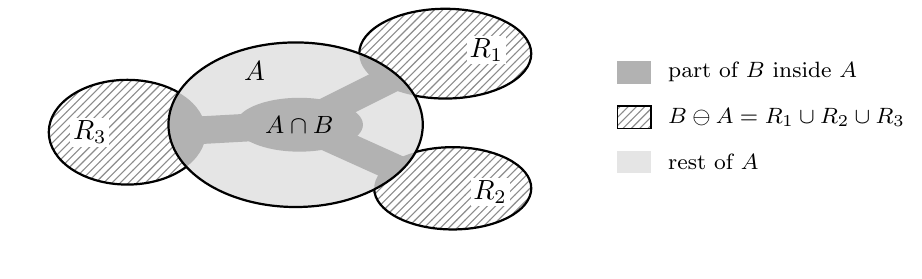
\begin{tikzpicture}[scale=0.95]
\draw[thick,pattern=north east lines,pattern color=black!45] (2.0,0.95) ellipse (1.15 and 0.6);
\draw[thick,pattern=north east lines,pattern color=black!45] (2.1,-0.85) ellipse (1.05 and 0.55);
\draw[thick,pattern=north east lines,pattern color=black!45] (-2.25,-0.1) ellipse (1.05 and 0.7);
\fill[gray!20] (0,0) ellipse (1.7 and 1.1);
\begin{scope}
\clip (0,0) ellipse (1.7 and 1.1);
\fill[gray!60] (2.0,0.95) ellipse (1.15 and 0.6);
\fill[gray!60] (2.1,-0.85) ellipse (1.05 and 0.55);
\fill[gray!60] (-2.25,-0.1) ellipse (1.05 and 0.7);
\fill[gray!60] (0.05,0) ellipse (0.85 and 0.36);
\draw[gray!60,line width=10pt,line cap=round] (0.05,0) -- (1.55,0.75);
\draw[gray!60,line width=10pt,line cap=round] (0.05,0) -- (1.6,-0.7);
\draw[gray!60,line width=10pt,line cap=round] (0.05,0) -- (-1.75,-0.1);
\end{scope}
\draw[thick] (0,0) ellipse (1.7 and 1.1);
\node at (-0.55,0.72) {$A$};
\node at (0.05,0) {\small $A\cap B$};
\node[fill=white,inner sep=1pt] at (2.55,1.0) {$R_1$};
\node[fill=white,inner sep=1pt] at (2.6,-0.9) {$R_2$};
\node[fill=white,inner sep=1pt] at (-2.75,-0.1) {$R_3$};
\fill[gray!60] (4.3,0.55) rectangle (4.75,0.85);
\draw[pattern=north east lines,pattern color=black!45] (4.3,-0.05) rectangle (4.75,0.25);
\fill[gray!20] (4.3,-0.65) rectangle (4.75,-0.35);
\node[anchor=west] at (4.85,0.7) {\footnotesize part of $B$ inside $A$};
\node[anchor=west] at (4.85,0.1) {\footnotesize $B\ominus A=R_1\cup R_2\cup R_3$};
\node[anchor=west] at (4.85,-0.5) {\footnotesize rest of $A$};
\end{tikzpicture}
\caption{Schematic picture of Lemma~\ref{L:complement}. The regular subcontinuum $B$ is the union of the three hatched regions and of the dark region inside $A$, which joins them; so $B$ is connected. When $\D(X)$ is countable, $B\rd A$ has finitely many components $R_1,\dots,R_k$; each is a regular subcontinuum and meets $A$.}\label{F:complement}
\end{figure}

\begin{lemma}[Complement lemma]\label{L:complement}
Let $\D(X)$ be countable, and let $A,B\in\D(X)$ with $A\cap B\neq\emptyset$ and $B\not\subseteq A$. Put $R=B\rd A$. Then:
\begin{enumerate}[label=\textup{(\arabic*)}]
\item\label{c1} $R$ is a nonempty regular closed set, $R\subseteq B$, $R\cap\intr A=\emptyset$, and $A\cup B=A\cup R$;
\item\label{c2} every component of $R$ meets $A$;
\item\label{c3} $R$ has finitely many components, and each of them is an element of $\D(X)$.
\end{enumerate}
\end{lemma}

\begin{proof}
\ref{c1} If $\intr B\subseteq A$ then $B=\cl\intr B\subseteq A$; so $\intr B\setminus A\neq\emptyset$ and $R\neq\emptyset$. The other assertions are in Lemma~\ref{L:rc}\ref{rc:basic}; note that $B\setminus A\subseteq R\subseteq B$ gives $A\cup B=A\cup R$.

\ref{c2} Suppose a component $C$ of $R$ misses $A$. By Lemma~\ref{L:components}\ref{comp:sep}, applied in the compact space $R$ to the closed set $A\cap R$, there is a relatively clopen subset $V$ of $R$ with $C\subseteq V$ and $V\cap A=\emptyset$. Let $Y=A\cup B=A\cup R$. The set $V$ is closed, and $Y\setminus V=A\cup(R\setminus V)$ is closed. Both are nonempty, so $Y$ is disconnected. But $Y$ is the union of two continua with a common point.

\ref{c3} Suppose $R$ has infinitely many components. By Lemma~\ref{L:components}\ref{comp:inf} there are pairwise disjoint nonempty relatively clopen subsets $V_1,V_2,\dots$ of $R$. Each $V_i$ is regular closed in $X$ by Lemma~\ref{L:rc}\ref{rc:clopen}. The components of $V_i$ are components of $R$, so by~\ref{c2} each of them meets $A$; hence $A\cup V_i$ is connected, and $C_i=A\cup V_i\in\D(X)$. Since $\intr B\setminus A$ is dense in $R$ and $V_i$ is relatively open in $R$, we can pick $x_i\in V_i\cap(\intr B\setminus A)$. Then $x_i\notin A$, and $x_i$ does not belong to the closed set $R\setminus V_i$, which contains $V_j$ for all $j\neq i$. Therefore $x_i\notin\cl(A\cup\bigcup_{j\neq i}C_j)$. The sequence $(C_i)$ is independent over $A$, and Lemma~\ref{L:independent} contradicts the countability of $\D(X)$.

So $R$ has finitely many components. Each is relatively clopen in $R$ by Lemma~\ref{L:components}\ref{comp:fin}, hence a nonempty regular closed set by Lemma~\ref{L:rc}\ref{rc:clopen}, and it is connected and compact.
\end{proof}

\subsection{An algebra of regular closed sets}

\begin{definition}
Let $\F(X)$ be the family consisting of the empty set and of all finite unions of elements of $\D(X)$.
\end{definition}

The members of $\F(X)$ are the regular closed sets that can be described by finitely many regular subcontinua. The complement lemma implies that this family is closed under the operations of Definition~\ref{D:ops}, which is what allows us to refine covers in Section~\ref{S:density}.

\begin{proposition}\label{P:algebra}
Let $\D(X)$ be countable and $F,G\in\F(X)$.
\begin{enumerate}[label=\textup{(\arabic*)}]
\item\label{a1} $F\cup G$, $F\rd G$ and $F\wedge G$ belong to $\F(X)$.
\item\label{a2} If $F\neq\emptyset$, then $F$ has finitely many components and each of them belongs to $\D(X)$.
\end{enumerate}
\end{proposition}

\begin{proof}
\ref{a2} A finite union of continua has finitely many components. Each is relatively clopen in the regular closed set $F$ (Lemmas~\ref{L:rc}\ref{rc:union} and~\ref{L:components}\ref{comp:fin}), hence regular closed by Lemma~\ref{L:rc}\ref{rc:clopen}.

\ref{a1} The case of unions is trivial. Let $A,B\in\D(X)$. If $A\cap B=\emptyset$ then $B\rd A=B$; if $B\subseteq A$ then $B\rd A=\emptyset$; otherwise $B\rd A\in\F(X)$ by Lemma~\ref{L:complement}. The first two identities of Lemma~\ref{L:rc}\ref{rc:ident} extend this to all of $\F(X)$: by the first, $F\rd A\in\F(X)$ for $F\in\F(X)$ and $A\in\D(X)$; by the second, removing a finite union $A_1\cup\dots\cup A_k$ amounts to removing $A_1,\dots,A_k$ successively. Finally $F\wedge G=F\rd(F\rd G)$ by the third identity.
\end{proof}

\subsection{Absorption}
We can now answer the question whether minimal regular subcontinua behave as indivisible pieces.

\begin{theorem}[Absorption]\label{T:absorption}
Let $\D(X)$ be countable and let $N$ be a minimal element of $\D(X)$. For every $A\in\D(X)$, either $N\subseteq A$ or $N\cap\intr A=\emptyset$. In particular, if $\intr A\cap\intr N\neq\emptyset$, then $N\subseteq A$.
\end{theorem}

\begin{proof}
Suppose $N\not\subseteq A$. If $A\cap N=\emptyset$ there is nothing to prove. Otherwise Lemma~\ref{L:complement} applies with $B=N$: the set $R=N\rd A$ is nonempty, and a component $R_1$ of $R$ is an element of $\D(X)$ with $R_1\subseteq R\subseteq N$. By minimality $R_1=N$, so $N\subseteq R$. Since $R\cap\intr A=\emptyset$, we get $N\cap\intr A=\emptyset$.
\end{proof}

\begin{corollary}\label{C:disjoint}
Let $\D(X)$ be countable. If $N\neq N'$ are minimal elements of $\D(X)$, then $N\cap\intr N'=\emptyset$. In particular $\intr N\cap\intr N'=\emptyset$.
\end{corollary}

\begin{proof}
By Theorem~\ref{T:absorption} with $A=N'$, either $N\subseteq N'$, which gives $N=N'$ by minimality of $N'$, or $N\cap\intr N'=\emptyset$.
\end{proof}

The proof of \cite[Proposition~3.15]{CORa} uses a maximal proper element of $\D(A\cup N)$ containing $A$, which exists when $\D(X)$ is discrete but need not exist when $\D(X)$ is merely countable. The complement lemma replaces that step. Example~\ref{E:cone} shows that Theorem~\ref{T:absorption} fails without a restriction on the size of $\D(X)$.

\subsection{Decreasing intersections}
If $A_1\subseteq A_2\subseteq\cdots$ are regular subcontinua, then $\cl\bigcup_nA_n$ is again one. Decreasing sequences are different: the intersection $K$ of regular subcontinua $A_1\supseteq A_2\supseteq\cdots$ is a continuum, but it may have empty interior, and when it has interior there is no general reason for it to contain a regular subcontinuum. The next lemma is the main technical step of the paper. It shows that, when $\D(X)$ is countable, the ``thick part'' $\cl\intr K$ of $K$ is as good as possible.

\begin{lemma}[Decreasing intersections]\label{L:decreasing}
Let $\D(X)$ be countable, let $A_1\supseteq A_2\supseteq\cdots$ be elements of $\D(X)$, and let $K=\bigcap_nA_n$. Then $\cl(X\setminus K)$ and $\cl\intr K$ belong to $\F(X)$. In particular, if $\intr K\neq\emptyset$, then $K$ contains an element of $\D(X)$.
\end{lemma}

The proof is by contradiction, and its idea is the following. If $\cl(X\setminus K)$ had infinitely many components, it would contain infinitely many pairwise disjoint relatively clopen pieces $V_i$. A whole piece $V_i$ cannot be deleted from $X$ without damage, because it reaches $K$. But $V_i$ is not contained in $K$, so some $A_{n_i}$ already misses part of it, and the part $O_i=V_i\setminus A_{n_i}$ can be deleted: what remains of $V_i$ lies in the regular subcontinuum $A_{n_i}$, which keeps it thick and keeps it attached to $K$. The sets $O_i$ are then blisters in the sense of Theorem~\ref{T:blister}. The two verifications in the proof, connectedness and regularity of $X$ minus finitely many $O_i$, make this precise.

\begin{proof}
The set $K$ is a continuum by Lemma~\ref{L:nested}. Let $R=\cl(X\setminus K)$, a regular closed set. We show that $R$ has finitely many components. This suffices: each component is then relatively clopen in $R$, hence regular closed, so $R\in\F(X)$; and $\cl\intr K=\cl(X\setminus R)=X\rd R\in\F(X)$ by Proposition~\ref{P:algebra}. The last assertion then follows from Proposition~\ref{P:algebra}\ref{a2}.

Suppose $R$ has infinitely many components. By Lemma~\ref{L:components}\ref{comp:inf} there are pairwise disjoint nonempty relatively clopen subsets $V_1,V_2,\dots$ of $R$. Write $V_i=R\cap W_i$ with $W_i$ open in $X$. Since $X\setminus K$ is dense in $R$, we can pick $x_i\in V_i\setminus K$, and then $n_i$ with $x_i\notin A_{n_i}$. Put
\[
O_i=V_i\setminus A_{n_i}.
\]
Because $X\setminus A_{n_i}\subseteq X\setminus K\subseteq R$, we have $O_i=W_i\setminus A_{n_i}$, which is open in $X$. The sets $O_i$ are nonempty, pairwise disjoint, and disjoint from $K$. For a finite set $F\subseteq\N$ let
\[
Y_F=X\setminus\bigcup_{i\in F}O_i .
\]
We shall prove that $Y_F\in\D(X)$ for every finite $F$. Theorem~\ref{T:blister}, applied with $A=X$, then gives $|\D(X)|=\cc$, a contradiction.

Fix a finite set $F$. We use the following observation.
\begin{itemize}
\item[$(\ast)$] For each $i$, the set $V_i\setminus K$ is relatively clopen in $X\setminus K$. Hence a connected subset of $X\setminus K$ is either contained in $V_i$ or disjoint from $V_i$.
\end{itemize}
Indeed $X\setminus K\subseteq R$ and $V_i$ is relatively clopen in $R$.

\emph{$Y_F$ is connected.} We have $K\subseteq Y_F$. It suffices to show that every $y\in Y_F\setminus K$ lies in a connected subset of $Y_F$ which meets $K$.

\emph{Case 1: $y\in V_i$ for some $i\in F$.} Since $y\notin O_i$, we have $y\in A_{n_i}$. Let $H$ be the component of $y$ in $A_{n_i}\setminus K$. By Lemma~\ref{L:bumping}, applied in the continuum $A_{n_i}$, the set $\cl H$ meets $K$. By $(\ast)$, $H\subseteq V_i$, so $\cl H\subseteq V_i\cap A_{n_i}$. This set misses $O_i$ and misses $O_j\subseteq V_j$ for $j\neq i$. So $\cl H\subseteq Y_F$.

\emph{Case 2: $y\notin V_i$ for all $i\in F$.} Let $H$ be the component of $y$ in $X\setminus K$. By $(\ast)$, $H$ misses $V_i$, hence $O_i$, for every $i\in F$. As the sets $O_i$ are open, $\cl H$ misses them too, so $\cl H\subseteq Y_F$; and $\cl H$ meets $K$ by Lemma~\ref{L:bumping}.

\emph{$Y_F$ is regular closed.} It is closed. If $F=\emptyset$ then $Y_F=X$. Otherwise let $n=\max\{n_i:i\in F\}$. Then $A_n\subseteq A_{n_i}$ misses $O_i$ for $i\in F$, so $A_n\subseteq Y_F$ and
\[
K\subseteq A_n=\cl\intr A_n\subseteq\cl\intr Y_F .
\]
Now let $y\in Y_F\setminus K$. If $y\in V_i$ for some $i\in F$, then $U=W_i\setminus K$ is an open neighbourhood of $y$ with $U\subseteq V_i$, and
\[
Y_F\cap U=U\setminus O_i=U\cap A_{n_i},
\]
because $U$ misses $V_j\supseteq O_j$ for $j\neq i$ and $O_i=W_i\setminus A_{n_i}$. Since $y\in A_{n_i}=\cl\intr A_{n_i}$, the point $y$ is a limit of points of the open set $U\cap\intr A_{n_i}\subseteq Y_F$. If $y\notin V_i$ for all $i\in F$, then $(X\setminus K)\setminus\bigcup_{i\in F}V_i$ is an open neighbourhood of $y$ contained in $Y_F$. In all cases $y\in\cl\intr Y_F$.
\end{proof}

\section{Density of the minimal elements}\label{S:density}

We now prove that, when $\D(X)$ is countable, minimal elements of $\D(X)$ are found near every point of $X$.

\begin{theorem}[Density]\label{T:density}
Let $\D(X)$ be countable. Then the union of the interiors of the minimal elements of $\D(X)$ is dense in $X$.
\end{theorem}

The idea is to cut $X$ along every element of $\D(X)$ in turn. After the $n$th cut, $X$ is covered by finitely many regular subcontinua (``cells''), each of which lies on one side of $D_n$: inside $D_n$ or inside $\cl(X\setminus D_n)$. One may think of the $n$th cut as deciding, for each cell, a yes-or-no question about $D_n$; a decreasing sequence of cells records a consistent list of answers for all elements of $\D(X)$. Following a decreasing sequence of cells leads to a continuum $K$ which lies on one side of every element of $\D(X)$; if $K$ has interior, Lemma~\ref{L:decreasing} provides a regular subcontinuum inside $K$, and $K$ is forced to coincide with it and to be minimal. Baire category then gives density, \emph{provided there are only countably many decreasing sequences of cells}. This is not automatic for a finitely branching tree. It follows from a linear ordering of the cells with connected initial unions: to each branch one can attach the regular subcontinuum lying ``to its left'', and at most two branches share the same one. See Figure~\ref{F:tree}.

\begin{figure}[ht]
\centering
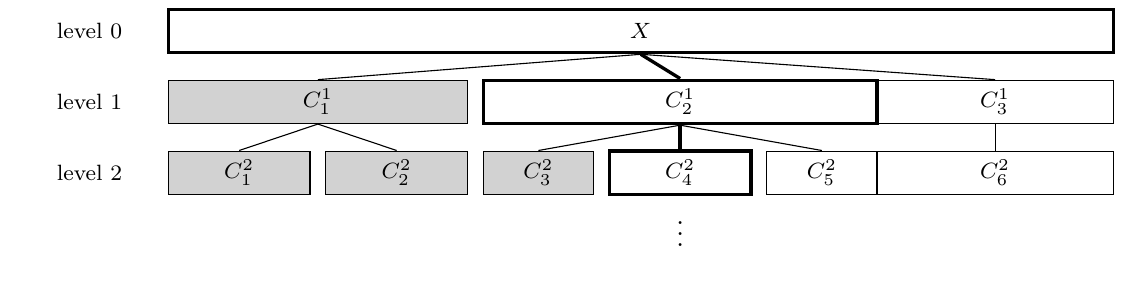
\begin{tikzpicture}[yscale=0.9,
cell/.style={draw,minimum height=5.5mm,inner sep=1pt,font=\footnotesize},
left/.style={cell,fill=gray!35},
br/.style={cell,very thick}]
\node[br,minimum width=120mm] (a) at (6,3) {$X$};
\node[left,minimum width=38mm] (b1) at (1.9,2) {$C^1_1$};
\node[br,minimum width=50mm] (b2) at (6.5,2) {$C^1_2$};
\node[cell,minimum width=30mm] (b3) at (10.5,2) {$C^1_3$};
\node[left,minimum width=18mm] (c1) at (0.9,1) {$C^2_1$};
\node[left,minimum width=18mm] (c2) at (2.9,1) {$C^2_2$};
\node[left,minimum width=14mm] (c3) at (4.7,1) {$C^2_3$};
\node[br,minimum width=18mm] (c4) at (6.5,1) {$C^2_4$};
\node[cell,minimum width=14mm] (c5) at (8.3,1) {$C^2_5$};
\node[cell,minimum width=30mm] (c6) at (10.5,1) {$C^2_6$};
\node at (-1,3) {\footnotesize level $0$};
\node at (-1,2) {\footnotesize level $1$};
\node at (-1,1) {\footnotesize level $2$};
\draw[very thick] (a.south) -- (b2.north);
\draw[very thick] (b2.south) -- (c4.north);
\draw (a.south) -- (b1.north);
\draw (a.south) -- (b3.north);
\draw (b1.south) -- (c1.north);
\draw (b1.south) -- (c2.north);
\draw (b2.south) -- (c3.north);
\draw (b2.south) -- (c5.north);
\draw (b3.south) -- (c6.north);
\node at (6.5,0.25) {$\vdots$};
\end{tikzpicture}
\caption{The tree of ordered covers in the proof of Theorem~\ref{T:density} (schematic). The cells of each level are listed from left to right, and every initial union is connected. Cells of the same level have disjoint interiors but may meet along their boundaries; the rectangles represent only their order. A branch $b$ is drawn in bold; the shaded cells are those placed before the cells of $b$, and the closure of their union is the set $L_b$.}\label{F:tree}
\end{figure}

\begin{proof}[Proof of Theorem~\ref{T:density}]
Enumerate $\D(X)=\{D_1,D_2,\dots\}$, with repetitions if $\D(X)$ is finite.

\medskip
\noindent\textbf{Step 1: ordered covers.} We construct, for each $n\ge0$, a finite list
\[
C^n_1,\ C^n_2,\ \dots,\ C^n_{k_n}
\]
of elements of $\D(X)$, the \emph{cells of level $n$}, with the following properties.
\begin{enumerate}[label=\textup{(P\arabic*)}]
\item\label{P1} The cells of level $n$ cover $X$ and have pairwise disjoint interiors.
\item\label{P2} For every $j\le k_n$ the initial union $P^n_j=C^n_1\cup\dots\cup C^n_j$ is connected.
\item\label{P3} Every cell of level $n+1$ is contained in a cell of level $n$, assigned to it as its \emph{parent}. The children of a cell cover it and occupy consecutive positions in the list, and if a cell $C$ is placed before a cell $C'$ at level $n$, then every child of $C$ is placed before every child of $C'$.
\item\label{P4} For $n\ge1$, every cell of level $n$ is contained in $D_n$ or in $\cl(X\setminus D_n)$.
\end{enumerate}
Level $0$ consists of the single cell $X$. Suppose level $n-1$ has been constructed, and let $C$ be one of its cells. By Proposition~\ref{P:algebra}, the sets $C\wedge D_n$ and $C\rd D_n$ belong to $\F(X)$, and their components are finitely many elements of $\D(X)$; these are the \emph{subcells} of $C$. By Lemma~\ref{L:rc}\ref{rc:basic} and~\ref{rc:split}, the subcells cover $C$, have pairwise disjoint interiors, and each is contained in $D_n$ or in $\cl(X\setminus D_n)$. The cells of level $n$ are the subcells of the cells of level $n-1$; they satisfy~\ref{P1} and~\ref{P4}, and it remains to order them.

Since the subcells of $C$ form a finite cover of the connected set $C$ by closed sets, their intersection graph is connected: otherwise $C$ would be the union of two disjoint nonempty closed sets. We process the cells of level $n-1$ in their order. If $C=C^{n-1}_1$, list the subcells of $C$ so that each one meets the union of the preceding ones; this is possible in a connected graph. If $C=C^{n-1}_j$ with $j>1$, let $P=P^{n-1}_{j-1}$. Both $P$ and $P\cup C=P^{n-1}_j$ are closed and connected by~\ref{P2}, so $P\cap C\neq\emptyset$ and some subcell of $C$ meets $P$. List first such a subcell, and then the remaining subcells of $C$ so that each one meets the union of $P$ and of the subcells of $C$ already listed. The list of level $n$ is the concatenation of these lists. Property~\ref{P3} holds by construction. An initial union at level $n$ is the union of some $P^{n-1}_{j-1}$ (empty if $j=1$) and of an initial part of the list of subcells of $C^{n-1}_j$, each member of which meets the union of what precedes it; so it is connected, and~\ref{P2} holds.

\medskip
\noindent\textbf{Step 2: branches.} A \emph{branch} is a sequence $b=(b_n)_{n\ge0}$ in which $b_n$ is a cell of level $n$ and $b_{n+1}$ is a child of $b_n$. For a branch $b$ let
\[
K_b=\bigcap_{n\ge0}b_n ,
\]
a continuum by Lemma~\ref{L:nested}. Every point $x\in X$ lies in some $K_b$: choose $b_0=X$ and, inductively, a child $b_{n+1}$ of $b_n$ containing $x$, which exists by~\ref{P3}. Hence
\begin{equation}\label{E:cover}
X=\bigcup_bK_b .
\end{equation}

\medskip
\noindent\textbf{Step 3: there are countably many branches.} By~\ref{P3}, if two branches $b,c$ satisfy $b_n\neq c_n$ and $b_n$ is placed before $c_n$, then $b_m$ is placed before $c_m$ for all $m\ge n$. So we may define $b<c$ if $b_n$ is placed before $c_n$ for some (equivalently, for every) $n$ with $b_n\neq c_n$; this is a linear order on the set of branches.

For a branch $b$ and $n\ge0$ let $U_n(b)$ be the union of the cells of level $n$ placed before $b_n$. This is an initial union, so it is empty or an element of $\D(X)$ by~\ref{P2}. By~\ref{P3} the children of the cells placed before $b_n$ are placed before $b_{n+1}$ and cover those cells; hence $U_n(b)\subseteq U_{n+1}(b)$. Let
\[
L_b=\cl\bigcup_{n\ge0}U_n(b).
\]
Then $L_b$ is empty or the closure of an increasing union of regular subcontinua, so $L_b\in\D(X)\cup\{\emptyset\}$.

We claim that $L_b\neq L_d$ whenever $b<c<d$ are three branches. Choose $n$ such that $b_n,c_n,d_n$ are pairwise distinct, say $b_n=C^n_i$, $c_n=C^n_j$, $d_n=C^n_k$; then $i<j<k$. First, $U_m(b)\subseteq P^n_i$ for every $m$. For $m\le n$ this holds because $U_m(b)\subseteq U_n(b)$. For $m>n$, a cell of level $m$ placed before $b_m$ has an ancestor of level $n$ which, by~\ref{P3}, is $b_n$ or is placed before $b_n$. As $P^n_i$ is closed, $L_b\subseteq P^n_i$. Second, $C^n_j\subseteq U_n(d)\subseteq L_d$. Third, $\intr C^n_j$ is disjoint from $P^n_i$: by~\ref{P1} it is disjoint from the interior of every other cell of level $n$, hence from every other cell of level $n$, since those are regular closed. As $\intr C^n_j\neq\emptyset$, we conclude $L_d\not\subseteq L_b$.

Thus the map $b\mapsto L_b$ from the set of branches to the countable set $\D(X)\cup\{\emptyset\}$ takes each value at most twice. So the set of branches is countable.

\medskip
\noindent\textbf{Step 4: a branch intersection with interior is a minimal element.} Let $b$ be a branch with $\intr K_b\neq\emptyset$. By Lemma~\ref{L:decreasing}, applied to the decreasing sequence $(b_n)$, there is $B\in\D(X)$ with $B\subseteq K_b$. Let $B'$ be any element of $\D(X)$ with $B'\subseteq K_b$, and choose $m\ge1$ with $B'=D_m$. By~\ref{P4}, $b_m\subseteq B'$ or $b_m\subseteq\cl(X\setminus B')$. The second alternative would give $B'\subseteq K_b\subseteq b_m\subseteq\cl(X\setminus B')$, which is impossible because the nonempty open set $\intr B'$ is disjoint from $\cl(X\setminus B')$. Hence
\[
B'\subseteq K_b\subseteq b_m\subseteq B',
\]
that is, $B'=K_b$. Applying this to $B'=B$ shows $K_b\in\D(X)$, and applying it to an arbitrary $B'$ shows that $K_b$ is a minimal element of $\D(X)$.

\medskip
\noindent\textbf{Step 5: Baire category.} Let $U$ be a nonempty open subset of $X$. By~\eqref{E:cover} and Step~3, $U$ is the union of the countably many relatively closed sets $U\cap K_b$. Since $U$ is a Baire space \cite[Theorem~8.4]{Kechris}, some $U\cap K_b$ has nonempty interior in $U$, hence in $X$. By Step~4 this $K_b$ is a minimal element of $\D(X)$, and $U$ meets its interior.
\end{proof}

\begin{remark}
Step~3 is the only place where the order of the cells is used. Unlike the results of Section~\ref{S:complements}, this proof uses the countability of $\D(X)$ directly and not through the counting principles of Section~\ref{S:obstructions}: in the enumeration on which the whole construction is based (Steps~1 and~4), in the bound on the number of branches (Step~3), and in the Baire category argument (Step~5).
\end{remark}

\section{\texorpdfstring{$\D$}{D}-atomic continua and the proof of the main theorems}\label{S:atomic}

\subsection{Atomic families}
The following definition isolates the conclusion of Theorems~\ref{T:absorption} and~\ref{T:density}.

\begin{definition}\label{D:atomic}
Let $X$ be a continuum. A family $\PP\subseteq\D(X)$ is an \emph{atomic family} for $X$ if
\begin{enumerate}[label=\textup{(A\arabic*)}]
\item\label{A1} \textup{(absorption)} for all $A\in\D(X)$ and $P\in\PP$, if $\intr A\cap\intr P\neq\emptyset$ then $P\subseteq A$;
\item\label{A2} \textup{(density)} the union of the interiors of the elements of $\PP$ is dense in $X$.
\end{enumerate}
The continuum $X$ is \emph{$\D$-atomic} if it has an atomic family. The elements of $\PP$ are called \emph{atoms}. For $A\in\D(X)$ we write $\PP(A)=\{P\in\PP:P\subseteq A\}$.
\end{definition}

Intuitively, a $\D$-atomic continuum is tiled, up to a nowhere dense remainder, by regular subcontinua that no regular subcontinuum can split. The chain of indecomposable continua in Example~\ref{E:chain} is a typical case: there the atoms are the links. The definition places no restriction on how atoms meet or accumulate, and the remainder $X\setminus\bigcup_{P\in\PP}\intr P$ may contain nondegenerate continua. Atoms are indivisible only relative to $\D(X)$: by Lemma~\ref{L:atomic} below an atom contains no proper regular subcontinuum of $X$, but it may contain many proper subcontinua with empty interior in $X$, as every nondegenerate indecomposable continuum does. We use the prefix $\D$ to avoid confusion with atomic maps and with other uses of the word ``atom'' in continuum theory. The arc is not $\D$-atomic (Example~\ref{E:arc}).

The next lemma shows that an atomic family is unique and that the pairwise disjointness of the interiors of the atoms need not be postulated.

\begin{lemma}\label{L:atomic}
Let $\PP$ be an atomic family for $X$.
\begin{enumerate}[label=\textup{(\alph*)}]
\item\label{at:disj} Distinct atoms have disjoint interiors; in particular $\PP$ is countable.
\item\label{at:rec} For every $A\in\D(X)$, the family $\PP(A)$ is nonempty and $A=\cl\bigcup\PP(A)$.
\item\label{at:min} $\PP$ is exactly the set of minimal elements of $\D(X)$.
\end{enumerate}
\end{lemma}

\begin{proof}
\ref{at:disj} If $P,Q\in\PP$ and $\intr P\cap\intr Q\neq\emptyset$, then~\ref{A1} gives $P\subseteq Q$ and $Q\subseteq P$. A separable metric space has no uncountable family of pairwise disjoint nonempty open sets.

\ref{at:rec} Let $W$ be a nonempty open subset of $\intr A$. By~\ref{A2} it meets $\intr P$ for some $P\in\PP$; then $\intr A\cap\intr P\neq\emptyset$, so $P\in\PP(A)$ by~\ref{A1}, and $W\cap P\neq\emptyset$. Thus $\bigcup\PP(A)$ is dense in $\intr A$, hence in $A$.

\ref{at:min} Let $P\in\PP$ and $B\in\D(X)$ with $B\subseteq P$. By~\ref{at:rec} there is $Q\in\PP$ with $Q\subseteq B\subseteq P$. The nonempty open set $\intr Q$ is contained in $P=\cl\intr P$, so it meets $\intr P$, and $Q=P$ by~\ref{at:disj}. Hence $B=P$, and $P$ is minimal. Conversely a minimal element $N$ contains an atom by~\ref{at:rec}, and equals it by minimality.
\end{proof}

The next proposition makes precise in what sense a $\D$-atomic continuum is determined, as far as $\D(X)$ is concerned, by its atoms.

\begin{proposition}\label{P:coding}
Let $\PP$ be an atomic family for $X$.
\begin{enumerate}[label=\textup{(\alph*)}]
\item\label{cod:bij} The map $A\mapsto\PP(A)$ is a bijection from $\D(X)$ onto the family of all nonempty sets $S\subseteq\PP$ such that $\cl\bigcup S$ is connected. Its inverse is $S\mapsto\cl\bigcup S$.
\item\label{cod:disc} For $P\in\PP$, the set $\{A\in\D(X):A\cap\intr P\neq\emptyset\}=\{A\in\D(X):P\subseteq A\}$ is open in $\D(X)$ and contains no atom other than $P$. In particular $\PP$ is a discrete subspace of $\D(X)$.
\end{enumerate}
\end{proposition}

\begin{proof}
We first note that if $P,Q\in\PP$ are distinct, then $Q\cap\intr P=\emptyset$: otherwise the open set $\intr P$ would meet $Q=\cl\intr Q$, hence $\intr Q$, contradicting Lemma~\ref{L:atomic}\ref{at:disj}.

\ref{cod:bij} By Lemma~\ref{L:atomic}\ref{at:rec}, for $A\in\D(X)$ the set $\PP(A)$ is nonempty and $\cl\bigcup\PP(A)=A$ is connected; so the map takes values in the stated family and is injective. Conversely let $S\subseteq\PP$ be nonempty with $A=\cl\bigcup S$ connected. Then $A$ is a regular closed continuum by Lemma~\ref{L:rc}\ref{rc:union}, so $A\in\D(X)$, and $S\subseteq\PP(A)$. If $P\in\PP\setminus S$, every element of $S$ is contained in the closed set $X\setminus\intr P$, hence so is $A$, and $P\not\subseteq A$. Thus $\PP(A)=S$.

\ref{cod:disc} The two sets are equal by~\ref{A1}, the first is open by Lemma~\ref{L:vietoris}\ref{v:meets}, and an atom $Q\neq P$ misses $\intr P$.
\end{proof}

\begin{remark}\label{R:notisolated}
Proposition~\ref{P:coding}\ref{cod:disc} does not say that an atom $P$ is an isolated point of $\D(X)$: the open set in~\ref{cod:disc} contains every regular subcontinuum that contains $P$. An atom can fail to be isolated only by being a limit of strictly larger regular subcontinua. In Example~\ref{E:chain} every atom is isolated; whether some atom must be isolated whenever $\D(X)$ is countable is Question~\ref{Q:isolated}.
\end{remark}

\subsection{Proof of Theorem~\ref{T:Gdelta}}
Let $\PP$ be an atomic family for $X$. By Lemma~\ref{L:atomic}\ref{at:rec}, a regular subcontinuum has two features: it treats every atom in an all-or-nothing way, and it has no part lying away from the atoms it contains. We express the first feature by a closed condition and the second by countably many open conditions.

Let $H$ be the set of all $A\in C(X)$ which contain each atom entirely or avoid its interior; that is, such that, for every $P\in\PP$,
\[
P\subseteq A\qquad\text{or}\qquad A\cap\intr P=\emptyset .
\]
By Lemma~\ref{L:vietoris}\ref{v:contains} and~\ref{v:meets}, both conditions define closed subsets of $C(X)$; so $H$ is closed in $C(X)$. If $A\in\D(X)$ and $A\cap\intr P\neq\emptyset$, then $\intr A\cap\intr P\neq\emptyset$ and $P\subseteq A$ by~\ref{A1}; so $\D(X)\subseteq H$.

For $A\in H$ and $P\in\PP$, the conditions ``$P\subseteq A$'' and ``$A\cap\intr P\neq\emptyset$'' are equivalent, because $\intr P\neq\emptyset$. The first is closed and the second is open. Hence
\begin{equation}\label{E:clopen}
\{A\in H:P\subseteq A\}\ \text{is clopen in }H\text{ for every }P\in\PP.
\end{equation}
A subcontinuum in $H$ may still fail to be regular, for instance by containing an arc that sticks out of the atoms it contains. The next condition excludes, up to an error $1/m$, any part of $A$ lying away from the atoms contained in $A$. For $m\in\N$ let $U_m$ be the set of all $A\in H$ for which there is a finite nonempty set $S\subseteq\PP$ with
\[
\bigcup S\subseteq A\subseteq N_{1/m}\Bigl(\bigcup S\Bigr).
\]
For a fixed $S$ the first condition is clopen in $H$ by~\eqref{E:clopen}, and the second is open by Lemma~\ref{L:vietoris}\ref{v:inside}. So $U_m$ is open in $H$. We claim that
\[
\D(X)=\bigcap_{m\in\N}U_m .
\]
This proves the theorem: each $U_m$ is the intersection of $H$ with an open subset of $C(X)$, and the closed set $H$ is itself a $G_\delta$ subset of the metric space $C(X)$; so $\bigcap_mU_m$ is a $G_\delta$ subset of $C(X)$.

Let $A\in\D(X)$ and $m\in\N$. By Lemma~\ref{L:atomic}\ref{at:rec}, the open sets $N_{1/m}(P)$, $P\in\PP(A)$, cover the compact set $A$; a finite subcover gives a finite nonempty $S\subseteq\PP(A)$ witnessing $A\in U_m$.

Conversely let $A\in\bigcap_mU_m$, and let $T$ be the union of all atoms contained in $A$. For each $m$ we have $A\subseteq N_{1/m}(T)$, so $A\subseteq\cl T$; and $\cl T\subseteq A$ because $A$ is closed. Thus $A=\cl T$ is a continuum which is the closure of a nonempty union of regular closed sets. By Lemma~\ref{L:rc}\ref{rc:union}, $A\in\D(X)$. \qed

\subsection{Proof of Theorems~\ref{T:structure} and~\ref{T:main}}

\begin{proof}[Proof of Theorem~\ref{T:structure}]
Parts~\ref{S1}, \ref{S2} and~\ref{S3} are Theorem~\ref{T:absorption}, Corollary~\ref{C:disjoint} and Theorem~\ref{T:density}. By~\ref{S1} and~\ref{S3}, $\M$ is an atomic family for $X$, and~\ref{S4} is Lemma~\ref{L:atomic}\ref{at:rec}.
\end{proof}

\begin{proof}[Proof of Theorem~\ref{T:main}]
By Theorem~\ref{T:structure}, $X$ is $\D$-atomic, so $\D(X)$ is a $G_\delta$ subset of the compact metric space $C(X)$ by Theorem~\ref{T:Gdelta}. A $G_\delta$ subset of a completely metrizable space is completely metrizable \cite[Theorem~3.11]{Kechris}.

Let $S$ be a nonempty subspace of $\D(X)$, and let $E$ be the closure of $S$ in $\D(X)$. Then $E$ is a nonempty, countable, completely metrizable space. If $E$ had no isolated point, each of its singletons would be closed and nowhere dense, and $E$ would be a countable union of nowhere dense sets, contradicting the Baire category theorem \cite[Theorem~8.4]{Kechris}. So $E$ has an isolated point $A$. As $\{A\}$ is open in $E$ and $S$ is dense in $E$, we have $A\in S$, and $A$ is isolated in $S$. Thus $\D(X)$ is scattered. If $W$ is a nonempty open subset of $\D(X)$, then $W$ has an isolated point, and this point is isolated in $\D(X)$ because $W$ is open; so the isolated points of $\D(X)$ are dense. Finally, a space homeomorphic to $\Q$ is countable and has no isolated point, so $\D(X)$ is never homeomorphic to $\Q$.
\end{proof}

\begin{corollary}\label{C:dichotomy}
For every metric continuum $X$, exactly one of the following holds: $|\D(X)|=\cc$, or $\D(X)$ is a countable, scattered, completely metrizable space and $X$ is $\D$-atomic.
\end{corollary}

\begin{proof}
$\D(X)$ is a Borel subset of the Polish space $C(X)$ \cite[Teorema~2.0.2]{Ram23}, so it is countable or of cardinality $\cc$ \cite[Theorem~13.6]{Kechris}. Apply Theorems~\ref{T:main} and~\ref{T:structure}.
\end{proof}

\begin{remark}
Theorem~\ref{T:main} also shows that the descriptive obstruction mentioned in the introduction is the true one: a hypothetical example for $\Q$ would need $\D(X)$ to be countable and not $G_\delta$ in $C(X)$, and these two requirements are incompatible. For uncountable hyperspaces $\D(X)$ need not be $G_\delta$; this is the case for $X=[0,1]^2$ \cite[p.~23]{Ram23}. By Theorem~\ref{T:Gdelta}, the square is not $\D$-atomic.
\end{remark}

\section{Examples and sharpness}\label{S:examples}

\begin{example}[The arc]\label{E:arc}
For $X=[0,1]$, $\D(X)$ is the set of nondegenerate closed subintervals. It has no minimal element, so by Lemma~\ref{L:atomic}\ref{at:min} the arc is not $\D$-atomic, and $|\D(X)|=\cc$. Thus the existence and density of minimal elements in Theorem~\ref{T:structure} require a hypothesis on $\D(X)$. Note that $\D([0,1])$ is open in $C([0,1])$; so the converse of Theorem~\ref{T:Gdelta} fails.
\end{example}

\begin{example}[A null chain; {\cite[Ejemplo~3.2.1]{Ram23}}]\label{E:chain}
Let $K_1,K_2,\dots$ be nondegenerate indecomposable continua in a metric space, converging in the Hausdorff metric to a singleton $\{p\}$ with $p\notin\bigcup_nK_n$, such that $K_n\cap K_{n+1}$ is a single point $q_n$ and $K_n\cap K_m=\emptyset$ for $|n-m|>1$. Let $X=\{p\}\cup\bigcup_nK_n$. Each $K_n$ is a regular subcontinuum of $X$, since $K_n\setminus\{q_{n-1},q_n\}$ is open in $X$ and dense in $K_n$. The family $\{K_n\}$ is an atomic family. Indeed, let $A\in\D(X)$ with $\intr A\cap\intr K_n\neq\emptyset$, and let $\rho\colon X\to K_n$ be the retraction that sends $K_1\cup\dots\cup K_{n-1}$ to $q_{n-1}$ (nothing if $n=1$) and $\{p\}\cup\bigcup_{m>n}K_m$ to $q_n$; it is continuous. If $A\not\subseteq K_n$, connectedness of $A$ forces $A$ to contain each of $q_{n-1},q_n$ on whose side it has points, so $\rho(A)=A\cap K_n$; in any case $A\cap K_n$ is a subcontinuum of $K_n$ with nonempty interior in $K_n$, hence equal to $K_n$, because a proper subcontinuum of an indecomposable continuum has empty interior. By Lemma~\ref{L:atomic}\ref{at:rec} and connectedness, the elements of $\D(X)$ are the finite chains $F_{n,m}=K_n\cup\dots\cup K_m$ ($n\le m$) and the tails $T_n=\{p\}\cup\bigcup_{k\ge n}K_k$. So $\D(X)$ is countably infinite. Its topology is easy to describe. For each $n$ the ``row'' $\{F_{n,m}:m\ge n\}\cup\{T_n\}$ consists of the elements containing $K_n$ but not $K_{n-1}$, so it is clopen in $\D(X)$ by~\eqref{E:clopen} below; within it, each $F_{n,m}$ is isolated and $F_{n,m}\to T_n$ as $m\to\infty$. Thus $\D(X)$ is a topological sum of countably many convergent sequences with their limits, which is the ordinal space $\omega^2$, as shown in~\cite{Ram23}. Every finite chain is an isolated point, the tails are the limit points, and the isolated points are dense, in accordance with Theorem~\ref{T:main}. As $n\to\infty$ both $F_{n,m}$ and $T_n$ converge in $C(X)$ to $\{p\}\notin\D(X)$, which illustrates Remark~\ref{R:complete}.
\end{example}

\begin{example}[Absorption can fail when $\D(X)$ is uncountable]\label{E:cone}
The idea is as follows. Take an indecomposable continuum $K$ which, in some open set, looks like a Cantor set of parallel arcs; the buckethandle is such a continuum. Cut a closed strip $B$ out of this family of arcs. By itself $B$ is far from connected. Now attach a cone over the set $E$ of right-hand endpoints of the arcs of $B$. The cone joins the arcs of $B$ to one another, so $B$ together with the cone is a regular subcontinuum which enters the interior of $K$ without containing $K$; and since the cone is attached to $K$ along a nowhere dense set, $K$ remains a minimal regular subcontinuum. Here is a concrete realisation, with coordinates that make the claims checkable. Let $C\subseteq[0,1]$ be the Cantor ternary set and let $K\subseteq\R^2\times\{0\}\subseteq\R^3$ be the Knaster buckethandle continuum: the union of the upper semicircles centred at $(\tfrac12,0)$ with endpoints in $C$, and of the lower semicircles centred at $(\tfrac{5}{2\cdot3^{n}},0)$, $n\ge1$, with endpoints in $C\cap[\tfrac{2}{3^{n}},\tfrac{1}{3^{n-1}}]$. It is a well-known indecomposable continuum; see \cite{Nadler}. Let $C'=\{c-\tfrac12:c\in C,\ c\ge\tfrac23\}$, a Cantor set of radii in $[\tfrac16,\tfrac12]$, and put
\[
B=\Bigl\{\bigl(\tfrac12+t,\sqrt{r^2-t^2},0\bigr):r\in C',\ |t|\le\tfrac1{12}\Bigr\},\qquad
E=\Bigl\{\bigl(\tfrac12+\tfrac1{12},\sqrt{r^2-\tfrac1{144}},0\bigr):r\in C'\Bigr\}.
\]
Thus $B\subseteq K$ is a Cantor set of arcs, $U=\{|t|<\tfrac1{12}\}\cap B$ is the intersection of $K$ with the open half-strip $\{|x-\tfrac12|<\tfrac1{12},\ y>0\}$, and $E$ is the set of right-hand endpoints of the arcs of $B$. Let $v=(1,1,1)$, let $\Gamma$ be the union of the segments from the points of $E$ to $v$, and let
\[
X=K\cup\Gamma,\qquad A=B\cup\Gamma .
\]
See Figure~\ref{F:cone}. The set $\Gamma$ is compact and connected, being the image of $E\times[0,1]$ under the continuous map $(e,s)\mapsto(1-s)e+sv$, all of whose segments contain $v$. Its points other than those of $E$ have positive third coordinate, so $K\cap\Gamma=E$, and $X$ is a continuum. The set $E$ is closed and nowhere dense in $K$: each of its points is the endpoint of an arc of $B$, hence a limit of points of $K\setminus E$.

\emph{$K$ is a minimal element of $\D(X)$.} The set $K\setminus E=X\setminus\Gamma$ is open in $X$ and, as just noted, dense in $K$; so $K\in\D(X)$. If $A'\in\D(X)$ and $A'\subsetneq K$, then $\intr A'$ is an open subset of $K$ contained in a proper subcontinuum of the indecomposable continuum $K$; so $\intr A'=\emptyset$, which is impossible.

\emph{$A\in\D(X)$.} The set $A$ is closed, and connected because every arc of $B$ meets $\Gamma$, which is connected. The set $U=(X\setminus\Gamma)\cap\{(x,y,z):|x-\tfrac12|<\tfrac1{12},\ y>0\}$ and the set $\Gamma\setminus E=X\setminus K$ are open in $X$ and contained in $A$, and $\cl U=B$, $\cl(\Gamma\setminus E)=\Gamma$. So $A=\cl\intr A$.

\emph{Absorption fails.} We have $\intr A\cap\intr K\supseteq U\neq\emptyset$, but $K\not\subseteq A$.

By Theorem~\ref{T:absorption}, $\D(X)$ must be uncountable. This is also seen directly: for $|s|<\tfrac1{12}$ the set $\{(\tfrac12+t,\sqrt{r^2-t^2},0)\in B:t\ge s\}\cup\Gamma$ is a regular subcontinuum of $X$. In this example $K\rd A$ is a nonempty regular closed proper subset of $K$; since $K$ is minimal, none of its nonempty relatively clopen subsets is connected (such a subset would be a regular subcontinuum properly contained in $K$), so it has infinitely many components, in contrast with Lemma~\ref{L:complement}.
\end{example}

\begin{figure}[ht]
\centering
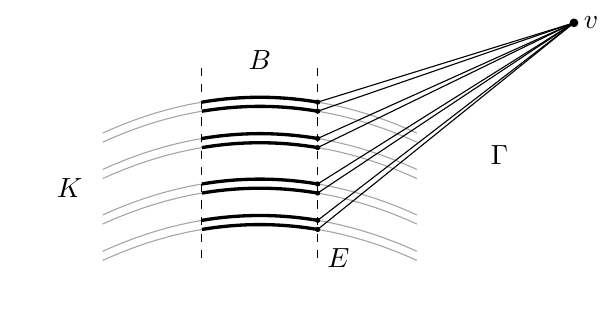
\begin{tikzpicture}[scale=1.05]
\foreach \r in {1.2,1.4,2.0,2.2,3.0,3.2,3.8,4.0}{
  \draw[gray!70] plot[domain=-1.9:1.9,samples=30] (\x,{0.55*\r+0.2-0.12*\x*\x});
}
\foreach \r in {1.2,1.4,2.0,2.2,3.0,3.2,3.8,4.0}{
  \draw[very thick] plot[domain=-0.7:0.7,samples=20] (\x,{0.55*\r+0.2-0.12*\x*\x});
  \draw (0.7,{0.55*\r+0.1412}) -- (3.8,3.3);
  \fill (0.7,{0.55*\r+0.1412}) circle (0.9pt);
}
\fill (3.8,3.3) circle (1.5pt) node[right] {$v$};
\node at (0,2.85) {$B$};
\node at (0.95,0.45) {$E$};
\node at (2.9,1.7) {$\Gamma$};
\node at (-2.3,1.3) {$K$};
\draw[dashed] (-0.7,0.45) -- (-0.7,2.75);
\draw[dashed] (0.7,0.45) -- (0.7,2.75);
\end{tikzpicture}
\caption{Example~\ref{E:cone} (schematic). Inside a chart of the buckethandle $K$, drawn in grey, the Cantor set of arcs $B$ is drawn in bold; the right-hand endpoints of its arcs are joined to a vertex $v$ outside the plane of $K$. The set $A=B\cup\Gamma$ is a regular subcontinuum whose interior meets the interior of the minimal element $K$ without containing it.}\label{F:cone}
\end{figure}

\begin{remark}[Dense-in-itself hyperspaces]
The continuum of~\cite{AdAirr} has $\D(X)$ homeomorphic to the irrationals. So an uncountable $\D(X)$ can be completely metrizable and have no isolated point; the countability hypothesis in the last part of Theorem~\ref{T:main} cannot be dropped.
\end{remark}

We end this section with a consequence of the unions principle for the order structure of $\D(X)$. It is not used in the proofs above, but it complements Theorem~\ref{T:main}: the main theorem says that a countable $\D(X)$ is scattered as a topological space, and the next proposition says that its chains are scattered as linear orders. The two notions are different, and neither statement implies the other in an obvious way.

\begin{proposition}\label{P:chains}
If $\D(X)$ is countable, then no subset of $\D(X)$ is ordered by inclusion in the order type of $\Q$.
\end{proposition}

\begin{proof}
Suppose $\{C_q:q\in\Q\}\subseteq\D(X)$ with $C_q\subsetneq C_{q'}$ for $q<q'$. For $r\in\R$ let $S_r=\cl\bigcup_{q<r}C_q$, the closure of the union of a chain of regular subcontinua; so $S_r\in\D(X)$. If $r<r'$, choose rationals $r<q<q'<r'$; then $S_r\subseteq C_q\subsetneq C_{q'}\subseteq S_{r'}$. So $r\mapsto S_r$ is injective and $|\D(X)|=\cc$.
\end{proof}

\section{Questions}\label{S:questions}

Theorem~\ref{T:main} restricts the countable spaces that can occur as $\D(X)$ to scattered completely metrizable ones. Which of them do occur is open. The finite case is settled in~\cite{CORa,AdAfin}; $\omega^2$ occurs (Example~\ref{E:chain}); the countable discrete space does not \cite[Theorem~3.25]{CORa}.

\begin{question}\label{Q:which}
Let $\D(X)$ be countably infinite.
\begin{enumerate}[label=\textup{(\alph*)}]
\item Which countable scattered completely metrizable spaces are homeomorphic to $\D(X)$ for some continuum $X$?
\item Is $\D(X)$ always locally compact?
\item Which countable ordinals $\alpha$, with the order topology, are homeomorphic to some $\D(X)$?
\end{enumerate}
\end{question}

Regarding~(c): an infinite $\D(X)$ is not compact \cite[Corollary~4.13]{Ord18}, so infinite successor ordinals do not occur; $\omega$ does not occur and $\omega^2$ does. By Theorem~\ref{T:structure} and Proposition~\ref{P:coding}, a countable $\D(X)$ is, as a set, the family of nonempty sets $S$ of minimal elements for which $\cl\bigcup S$ is connected. This describes the elements of $\D(X)$ combinatorially, but not its topology: by~\eqref{E:clopen} the correspondence $A\mapsto\PP(A)$ is continuous into the Cantor cube $2^{\PP}$, and we do not know when it is a homeomorphism onto its image. The answer depends on how the atoms are placed in $X$, for instance on whether their diameters tend to zero.

\begin{question}\label{Q:isolated}
Let $\D(X)$ be countably infinite. Is some minimal element of $\D(X)$ an isolated point of $\D(X)$?
\end{question}

Theorem~\ref{T:main} gives a dense set of isolated points of $\D(X)$, and Proposition~\ref{P:coding}\ref{cod:disc} shows that the set $\M$ of minimal elements is a discrete subspace of $\D(X)$. Neither statement produces a minimal element that is isolated in $\D(X)$. As explained in Remark~\ref{R:notisolated}, the issue is not accumulation of other minimal elements but approximation of a minimal element $N$ by strictly larger regular subcontinua, which by Lemma~\ref{L:atomic}\ref{at:rec} are closures of unions of $N$ with other minimal elements lying close to $N$. A considerably longer combinatorial argument, obtained during the development of this work, indicates that this cannot happen at every minimal element, so that the answer is yes. It is not needed here and has not been checked to the standard of the present paper, so we state the problem as a question; the argument is recorded in a development report available from the author.

\begin{question}\label{Q:polish}
Characterise the continua $X$ for which $\D(X)$ is a $G_\delta$ subset of $C(X)$.
\end{question}

Being $\D$-atomic is sufficient by Theorem~\ref{T:Gdelta} and not necessary by Example~\ref{E:arc}; the square is a continuum for which $\D(X)$ is not $G_\delta$ \cite[p.~23]{Ram23}.

\begin{question}\label{Q:absorb}
For which continua do the minimal elements of $\D(X)$ have the absorption property of Theorem~\ref{T:absorption}? Is there a natural condition on $X$, weaker than countability of $\D(X)$, under which regularised differences of regular subcontinua have finitely many components?
\end{question}

Example~\ref{E:cone} shows that some condition is needed. One sufficient condition is already contained in the proofs: Lemma~\ref{L:complement}, Proposition~\ref{P:algebra} and Theorem~\ref{T:absorption} use only that $X$ has no independent family in the sense of Definition~\ref{D:independent}. By Remark~\ref{R:arc} this condition is strictly weaker than countability of $\D(X)$; in the arc it holds, and absorption holds vacuously. What is open is a characterisation: we do not know a geometric description of the continua without independent families, nor whether absorption can hold in the presence of independent families.

\section*{Formalization in Lean 4}

The theorems of this paper have been formalized in Lean~4 \cite{Lean4} with the library Mathlib \cite{Mathlib}. The development is available at
\begin{center}
\url{https://github.com/LucasAlves8Sp/On-the-Structure-of-Countable-Hyperspaces-of-Regular-Subcontinua}
\end{center}
and was compiled with Lean \texttt{v4.35.0-rc2} and the Mathlib release of the same tag.

\emph{What is formalized.} Theorems~\ref{T:main}, \ref{T:structure} and~\ref{T:Gdelta}, Lemma~\ref{L:independent}, Theorem~\ref{T:blister}, Lemma~\ref{L:complement}, Proposition~\ref{P:algebra}, Theorem~\ref{T:absorption}, Corollary~\ref{C:disjoint}, Lemma~\ref{L:decreasing}, Theorem~\ref{T:density}, Lemma~\ref{L:atomic}, Proposition~\ref{P:coding}, Corollary~\ref{C:dichotomy} and Proposition~\ref{P:chains}, each with the hypotheses stated here and no additional one. In particular the file \texttt{Challenge.lean} contains the statement that there is no metric continuum $X$ with $\D(X)$ homeomorphic to $\Q$. The hyperspace $C(X)$ is modelled as the subspace of connected members of Mathlib's hyperspace of nonempty compact sets, whose topology is that of the Hausdorff metric. Every formal proof is complete, uses no axiom beyond the three standard ones of Lean with classical logic (\texttt{propext}, \texttt{Classical.choice}, \texttt{Quot.sound}), and was accepted by the Lean kernel and by the independent proof checkers run through the tool Comparator. The repository records exactly which checks were run and under which conditions.

\emph{What is not formalized.} Examples~\ref{E:arc}, \ref{E:chain} and~\ref{E:cone}, the remarks, and Lemmas~\ref{L:components} and~\ref{L:bumping} in the form stated here. The correspondence between the formal statements and the statements of this paper has so far been checked only by the AI system that wrote them.

\emph{Relation to the written proofs.} The formal proofs establish the statements above, but they do not follow the written proofs step by step. They do not use boundary bumping (Lemma~\ref{L:bumping}): connectedness is handled through separations by closed sets. Lemma~\ref{L:components} is replaced by a single dichotomy: a closed set is a finite union of connected relatively clopen subsets, or it contains infinitely many pairwise disjoint nonempty relatively clopen subsets. In Theorem~\ref{T:density} the tree of ordered covers is replaced by a sequence of finite families of pairs $P\subseteq P'$ of nested sets. The fact that $\D(X)$ is a Borel subset of $C(X)$, cited from \cite{Ram23} in the proof of Corollary~\ref{C:dichotomy}, is proved in the formalization. The formalization also shows that Proposition~\ref{P:algebra}\ref{a2} does not need the hypothesis that $\D(X)$ is countable.

\section*{Declaration of AI assistance}

The author used Fable~5.2 (Claude Fable~5.2, Anthropic) and ChatGPT-Astra extensively during the development of this work. These systems assisted with mathematical exploration, the formulation and development of proofs, theorem verification, proofreading, manuscript drafting, and editorial revision. In particular, the statements and proofs in this paper were proposed, developed and cross-checked in interaction with these systems, and the manuscript was drafted with their assistance.

The models involved in obtaining the results were Opus~5.5, Fable~5.2 and ChatGPT-Astra. Fable~5.2 carried out the main research. ChatGPT-Astra rechecked the arguments, compared them with the literature and re-derived the results. The author conducted the investigation: he chose the questions to be answered in view of the obstructions met in proving the result, redirected the search for results, and edited and checked the text. The literature search underlying the statements about prior work was carried out with the same assistance on November~10, 2026; it found no earlier resolution of the rational case of Question~\ref{Q:main}.

The Lean code of the formalization described in the previous section, both statements and proofs, was written by Fable~5.2 at the author's request.

The author takes responsibility for the content of the paper.

\bibliographystyle{amsplain}
\bibliography{refs}

\end{document}
